\documentclass[tikz,border=10pt]{standalone}
\usepackage{tikz}

\begin{document}

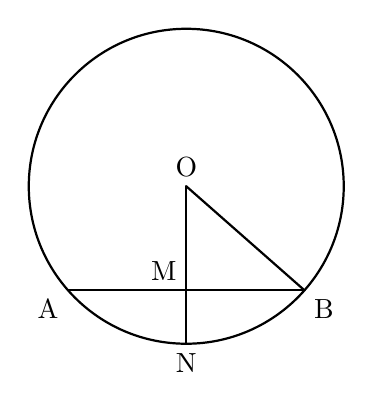
\begin{tikzpicture}[scale=1, line cap=round, line join=round]

% Define Center
\coordinate (O) at (0,0);

% Draw Circle with radius 2
\draw[thick] (O) circle (2);

% Define points for the chord AB
% Placing chord in the lower half based on image 10 11.png
\coordinate (A) at (-1.5, -1.32);
\coordinate (B) at (1.5, -1.32);

% Define M (midpoint of AB) and N (point on circumference)
\coordinate (M) at (0, -1.32);
\coordinate (N) at (0, -2);

% Draw line segments
\draw[thick] (A) -- (B);       % Chord AB
\draw[thick] (O) -- (N);       % Segment ON passing through M
\draw[thick] (O) -- (B);       % Radius OB

% Label points exactly as shown in the image
\node[above] at (O) {O};
\node[below left] at (A) {A};
\node[below right] at (B) {B};
\node[above left] at (M) {M};
\node[below] at (N) {N};

\end{tikzpicture}

\end{document}
